\section{Theoretical results}
\label{sec:theoryresults}
In this section, we prove for linear functions $f_\theta(x) =
\theta^\top x$ that  in the case of directed attacks, robust
generalization deteriorates with increasing $\epstrain$.
The proof, albeit in a simple setting, provides
explanations for why adversarial training fails in the
high-dimensional regime for such attacks.
%\fy{see my comment - keep only if true}
%In particular, in Appendix
%\ref{sec:app_theorycs} we show that the intuition also carries over to
%models that learn the features, such as a two-layer networks, which suggests that the intuition carries over to the real-world experiments in Section 5 as well.
% \fy{which
  %suggests that this could be the reason behind the phenomena on
  %eal-world NN experiments in Section bla as well.}


\subsection{Setting}
\label{logreg_linear_model}

We now introduce the precise linear setting used in our theoretical results.

%\fy{Jacob - these two paragraphs were saying the exact same thing.. ---} 

%% We start our exposition with the simplest setting: high-dimensional
%% linear classification, where the ground truth and hypothesis class are
%% given by linear functions $f_\theta(x) = \theta^\top x$ and the sample
%% size is lower than the ambient dimension. Albeit simple, the
%%  gives intuitive
%% insights that transfer to more complicated setting, which we discuss in the section on real-world experiments and in Appendix \ref{sec:app_theorycs}.

%% present details on the distribution, perturbation sets and
%% estimators when the ground truth and search space are linear
%% classifiers based on linear functions $f_\theta(x) = \theta^\top x$.

\paragraph{Data model}
%For Sections \ref{logreg_linear_model}, \ref{logreg_proof_sketch} and
%\ref{logreg_main_theorem}
In this section, we assume that the ground truth and hypothesis class
are given by linear functions $f_\theta(x) = \theta^\top x$ and the
sample size $\numsamp$ is lower than the ambient dimension $\dims$.  In
particular, the generative distribution $\prob_\sigsep$ is similar to
\cite{tsipras19, kolter19}: The label $y \in \{+1, -1\}$ is drawn with
equal probability and the covariate vector is sampled as $x =
[y\frac{\sigsep}{2}, \xnonsig]$ with the random vector $\xnonsig \in
\R^{\dims-1}$ drawn from a standard normal distribution,
i.e. $\xnonsig \sim \Normal(0, \sigma^2 I_{d-1})$. We would like to
learn a classifier that has low robust error by using a dataset
$\data = {(x_i, y_i)}_{i=1}^n$ with $\numsamp$ i.i.d. samples from
$\prob_{\sigsep}$.

Notice that the distribution $\prob_{\sigsep}$ is noiseless: for a given input
$x$, the label $y = \sign(\xind{1})$ is deterministic. Further, the
optimal linear classifier (also referred to as the \emph{ground
  truth}) is parameterized by $\thetatrue = e_1$.\footnote{Note that the result more generally holds for non-sparse models that are not axis aligned by way of a simple rotation $z = U x$. In that case the distribution is characterized by $\thetastar = u_1$ and a rotated Gaussian in the $\dims-1$ dimensions orthogonal to $\thetastar$.} By definition, the ground truth is
robust against all consistent perturbations and hence the optimal
robust classifier.
% robust against all perturbations.  - what does this mean?
%\fy{this is by definition of robust} to any sample of the distribution.

%% We would like to \fy{why? couldn't the optimal robust classifier
%%   for some particular perturbation be in some set, i.e. not a singleton?} 
%% estimate $\thetatrue$ with a high accuracy by using a dataset $\data =
%% {(x_i, y_i)}_{i=1}^n$ with $\numsamp$ i.i.d. samples from $\prob_{\sigsep}$.


%\fy{it's an
%example of a structured ground truth that has hope to be recovered in the
%high-dimensional settings $d\gg n$}
%\fy{could cite some}.


\paragraph{\nameofattackscapital}  
The focus in this paper lies on consistent \nameofattacks that by
definition efficiently concentrate their attack budget in the
direction of the signal.  For our linear setting, we can model such
attacks by  additive perturbations in the first dimension
\begin{equation}
  \label{eq:linfmaxpert}
  \pertset{x}{\eps} = \{x'=x+\delta  \mid \delta = \beta e_1 \text{ and } -\eps \leq \beta\leq \eps\}.
\end{equation}
Note that this attack is always in the direction of the true signal dimension, i.e. the ground truth. Furthermore, when  $\epsilon < \frac{r}{2}$, it is a consistent \nameofattack.
Observe how this is different from $\ell_p$ attacks - an $\ell_p$ attack, depending on the model, may add a perturbation that only has a very small component in the signal direction. 
%% that specifically attack the signal dimension in the
%% ground truth, i.e. move the samples closer to the decision
%% boundary. For our setting, this includes additive perturbations in the
%% first dimension
%% \begin{equation}
%%   \label{eq:linfmaxpert}
%%   \pertset{x}{\eps} = \{x'=x+\delta  \mid \delta = \beta e_1 \text{ and } -\eps \leq \beta\leq \eps\}.
%% \end{equation}
%% When the ground truth is $e_1$, the signal is in the first component -
%% therefore, a transformation that adds a vector in the direction of
%% $e_1$ reduces the distance of a point $x$ to the optimal decision boundary, which means that the perturbed sample is harder to distinguish from a sample that is of the other class then the original sample. Thus, the perturbation is ``signal-attacking''.

%% Throughout, we consider perturbation sizes with $\epsilon < \frac{r}{2}$, so
%% that the perturbations are consistent.  Note that this particular
%% perturbation could result from directly searching in the set of
%% perturbations along $e_1$ or by considering $l_1$-balls, because
%% $l_1$-ball constrained perturbations find sparse solutions. Our
%% results hold for both kinds of perturbation sets.



\paragraph{Robust max-$\ell_2$-margin classifier}

%For interpolators, it is important to study the inductive or implicit
%bias of popular algorithms. 
A long line of work studies the implicit bias of interpolators
that result from applying stochastic gradient descent on the logistic loss until convergence \cite{liu20, Ji19, Chizat20, nacson19}.
For linear models, we obtain the $\epstrain$-robust maximum-$\ell_2$-margin solution (\emph{robust max-margin} in short) 
\begin{equation}
  \label{eq:maxmargin}
  \thetahat{\epstrain} := \argmax_{\|\theta\|_2\leq 1} \min_{i\in [n], x_i' \in \pertset{x_i}{\epstrain}} y_i \theta^\top x_i'.
\end{equation}
This can for example be shown by a simple rescaling
argument using Theorem 3.4 in \cite{liu20}.  Even though our result is proven for the max-$\ell_2$-margin classifier,
it can easily be extended to other interpolators.
%% that
%% adversarial training may also fail to increase
%% %\fy{shouldn't we be able to show hurt??: fail to increase, yes!} 
%% robust generalization for any other baseline classifier such as the max-$\ell_1$-margin classifier (as a result of AdaBoost \cite{telgarsky13}).
%% we discuss the
%% particular implicit bias of gradient descent, adversarial training can also fail to increase robust generalization for any other baseline classifier such as the max-$\ell_1$-margin classifier that we briefly discuss in Section~\ref{sec:discussion}. We leave a rigorous proof and detailed analysis for future work.

%\fy{note for Julia: standard training corresponds to the usual max-$\ell_2$ margin solution...}
%% Our main goal is to assess the robust test performance of classifiers
%% obtained using standard adversarial training procedures in practice.
%% In particular a popular loss function to choose in the empirical risk~\eqref{eq:sgdrob} is $\loss(z) = \log (1+ \E^{-z})$ and one popular algorithm
%% to minimize it is (stochastic) gradient descent.
%% A long line of work shows the implicit bias of gradient descent on the logistic loss \fy{nati, matus, chizat, ... } for a variety of models. 

%% that is perfectly robust and accurate classifier on the training
%% set. If one runs adversarial training on the logistic loss~\eqref{eq:sgdrob} with $\loss(z) = \log (1+ \E^{-z})$,
%% BLABLA show that at convergence, we obtain
%% In practice, one can obtain such classifiers by running an
%% iterative algorithm until convergence.
%% %% We study interpolating estimators because \jc{they are widely used}.
%% %% In Section \ref{logreg_main_theorem} we first consider linear functions $f_\theta(x) = \theta^\top x$.
%% In particular,  \cite{Li20} show that gradient descent on the logistic loss~\eqref{eq:emploss} until convergence converges to

\begin{figure*}[!t]
  \centering
\begin{subfigure}[b]{0.3\textwidth}
  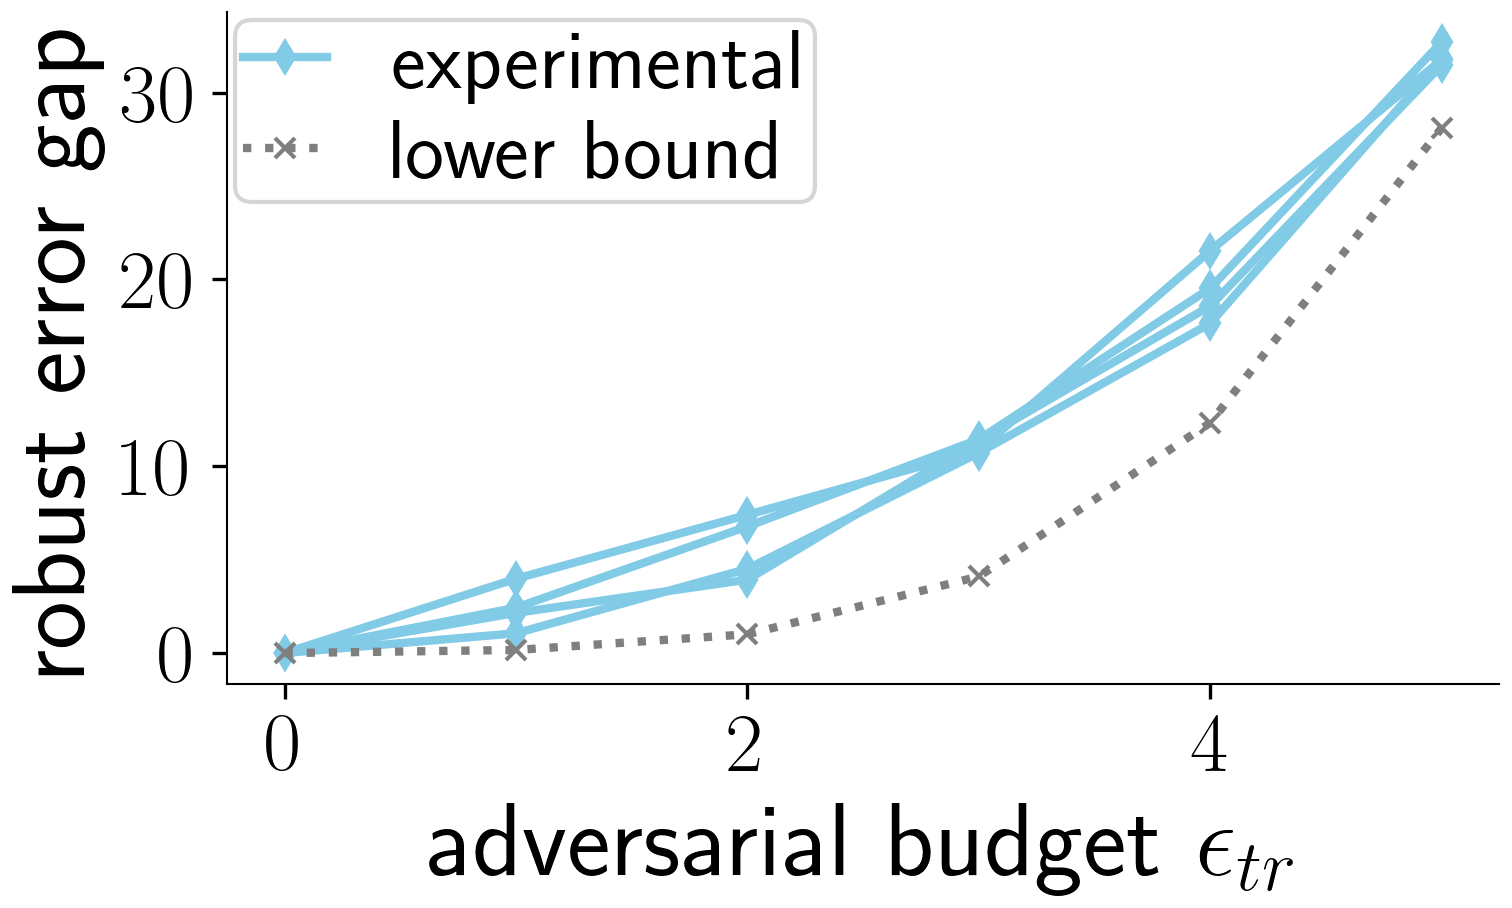
\includegraphics[width=0.99\linewidth]{plotsAistats/gap_lower_final_main_theorem.png}
  \caption{Robust error increase with $\epstrain$}
  \label{fig:main_lower_bound_eps}
\end{subfigure}
\begin{subfigure}[b]{0.3\textwidth}
  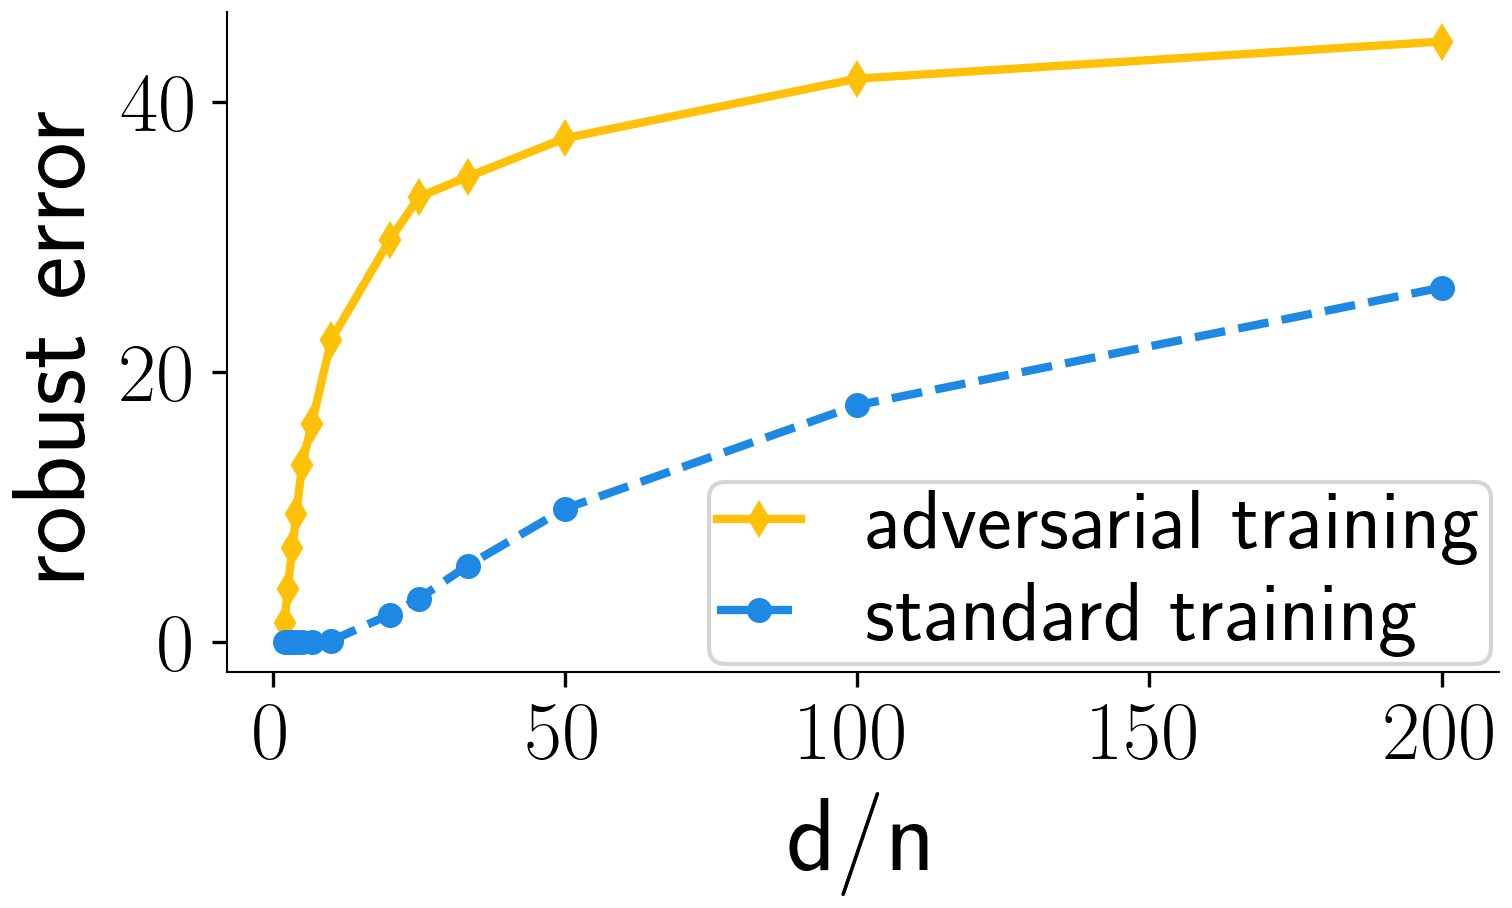
\includegraphics[width=0.99\linewidth]{plotsAistats/robust_error_ST_AT.png}
  \caption{Standard-adversarial training}
  \label{fig:main_numobs}
\end{subfigure}
\begin{subfigure}[b]{0.3\textwidth}
  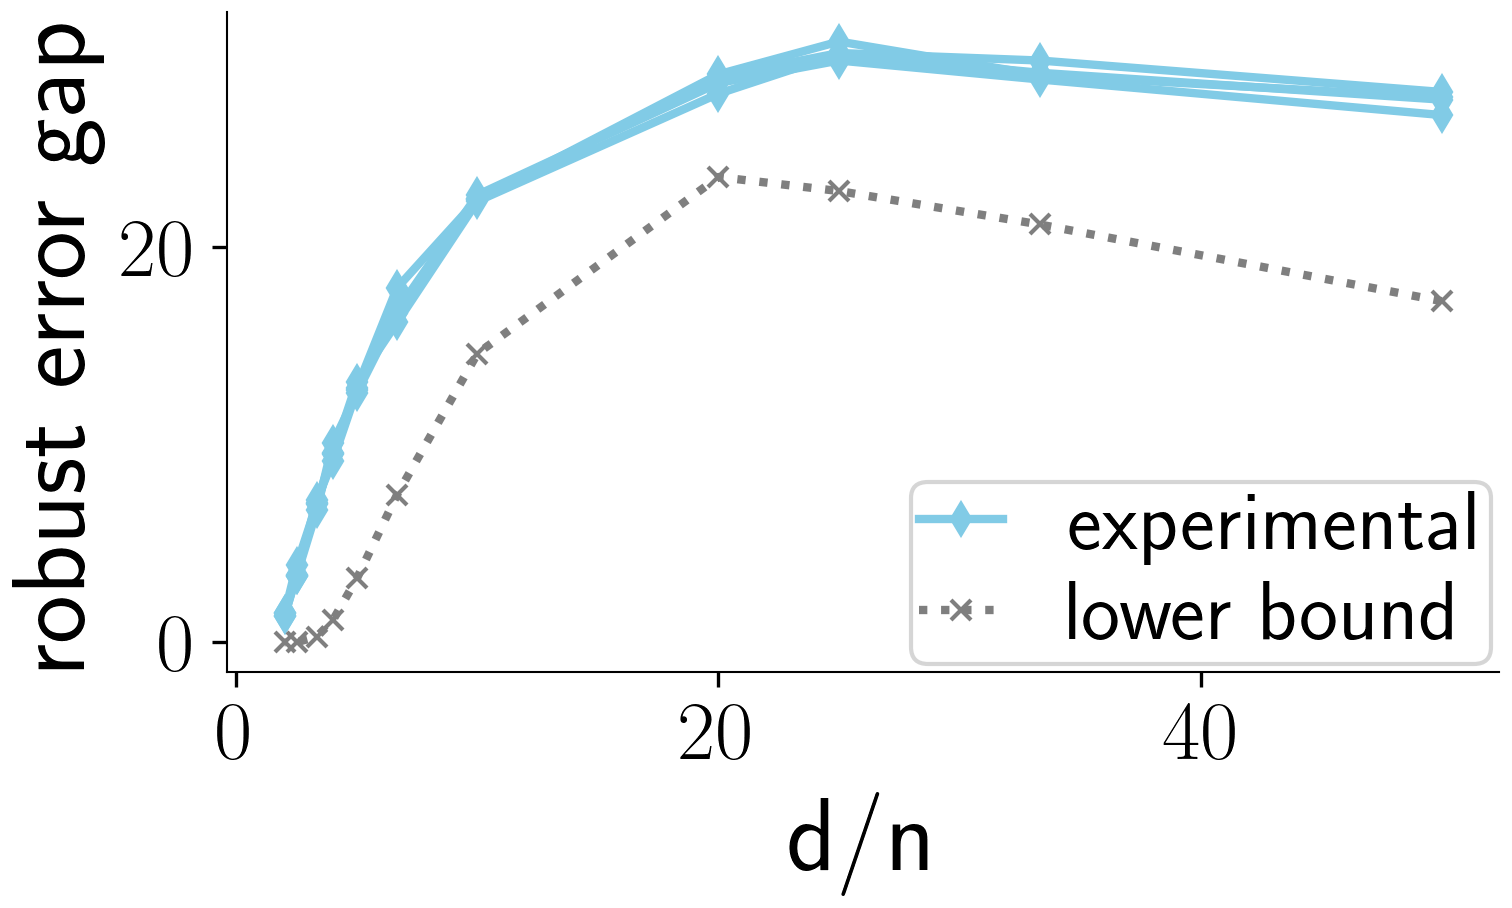
\includegraphics[width=0.99\linewidth]{plotsAistats/gap_final_good_colours.png}
  \caption{Effect of over-parameterization}
  \label{fig:main_numobs_bound}
\end{subfigure}
\caption{Experimental verification of Theorem \ref{thm:linlinf}.
(a) We set $\dims = 1000$, $\sigsep = 12$, $\numsamp = 50$ and plot the robust error gap between standard and adversarial training with increasing adversarial budget $\epstrain$ of $5$ independent experiments. For comparison, we also plot the lower bound given in Theorem \ref{thm:linlinf}. In (b) and (c), we set $\dims = 10000$ and vary the number of samples $\numsamp$. (b) We plot the robust error of standard and adversarial training ($\epstrain = 4.5$). (c) We compute the error gap and the lower bound of Theorem \ref{thm:linlinf}. For more experimental details see Appendix~\ref{sec:logregapp}.}
  \vspace{-0.2in}
\label{fig:main_theorem}
\end{figure*}

\subsection{Main results}
\label{logreg_main_theorem}


We are now ready to characterize the
$\epstest$-robust error as a function of $\epstrain$, the separation
$\sigsep$, the dimension $\dims$ and sample size $\numsamp$ of the
data. In the theorem statement we use the following quantities
\begin{align*}
      \varphimin &= \frac{\mixvar}{r/2-\epstest}  \left(  \sqrt{\frac{\dims-1}{\numsamp}} - \left(1 + \sqrt{\frac{2 \log (2/\delta)}{\numsamp}}\right)\right)\\
      \varphimax &= \frac{\mixvar}{r/2-\epstest}  \left(  \sqrt{\frac{\dims-1}{\numsamp}} + \left(1 + \sqrt{\frac{2 \log (2/\delta)}{\numsamp}}\right)\right)
\end{align*}
that arise from concentration bounds for the singular values of the random data matrix. Further, let $\epscutoff := \frac{\sigsep}{2} - \frac{\varphimax}{\sqrt{2}}$ and denote by
%% and refer to $\normaldens(x; \randvarphi) =  \frac{1}{\sqrt{2\pi} \randvarphi}\E^{-\frac{x^2}{\randvarphi^2}} $ as the density function of a Gaussian distribution with mean zero and variance $\randvarphi$.
 $\Phi$ the cumulative distribution function of a standard normal.
\begin{theorem}
  \label{thm:linlinf}
  %% The following results hold when the $d-1$ non-signal dimensions are linearly separable, which is true almost surely when
  Assume $d-1>n$. 
  For any $\epstest \geq 0$, the $\epstest$-robust error on test samples from $\prob_{\sigsep}$ with $2 \epstest < \sigsep$ and perturbation sets in Equation~\eqref{eq:linfmaxpert} and~\eqref{eq:l1maxpert}, the following holds:
  \begin{enumerate}
  \item
    %% Almost surely (over the draw of the dataset $\data$ with samples from $\prob_\sigsep$),
    %% \fy{If the $d-1$ non-signal dimensions are linearly separable,
      The $\epstest$-robust error of the $\epstrain$-robust max-margin estimator reads
    \begin{equation}
      \roberr{\thetahat{\epstrain}} = \Phi \left( -\frac{\left( \frac{r}{2}-\epstrain \right) }{\randvarphi} \right)
    \end{equation}
    %% \begin{equation}
    %%   \roberr{\thetahat{\epstrain}} = \Phi \left( -\frac{\left( \frac{r}{2}-\epstrain \right) \left(\frac{r}{2}-\epstest \right)  }{\mixvar \marginnonsig} \right)
    %% \end{equation}
    for a random quantity $\randvarphi>0$ depending on $\sigma, \sigsep,\epstest$, which is a strictly increasing function with respect to $\epstrain$.
    %% We refer to $ \frac{d \roberr{\thetahat{\epstrain}} }{d \epstrain} = \normaldens(\sigsep/2 - \epstrain ; \randvarphi)$ as the sensitivity of the drop of the robust error to AT perturbation set size $\epstrain$.
    %% \fy{with this notation the dependence on $\epstest$ and everything is lost, but maybe ok?i.e. get rid of of $\epstest$ as argument?}
    %% \fy{this feels to me more like part of the interpretatin since its trivial statement...} The sensitivity of the drop of the robust error to AT perturbation set size $\epstrain$ is captured by the derivative
    %% \begin{equation*}
    %%   \frac{d \roberr{\thetahat{\epstrain}} }{d \epstrain} = \frac{1}{\sqrt{2\pi} \randvarphi}\E^{-\frac{(\frac{\sigsep}{2} - \epstrain)^2}{\randvarphi^2}} 
    %% \end{equation*}
     
  %% \item If $\epstrain \leq \frac{\sigsep}{2} - \frac{\varphimax}{\sqrt{2}}$ , then with probability at least $1-\delta$, we further have $\varphimin \leq \randvarphi\leq \varphimax$ and  the following lower bound on the robust error drop
  %%   \begin{multline*}
  %%     \roberr{\thetahat{\epstrain}} - \roberr{\thetahat{0}} \geq 
  %%     %\int_{r/2-\epstrain}^{r/2} \frac{1}{\sqrt{2\pi}\varphi} \E^{- \frac{x^2 }{\varphi^2}} \d x
  %%     \Phi \left(\frac{r/2}{\varphimin} \right) - \Phi \left(  \frac{r/2 -\epstrain}{ \varphimin} \right).
  %%   \end{multline*}

  \item
    %\fy{alternative statement cause $\epstrain<$ doesn't make sense if you want to show AT sucks (i.e. higher should be worse)}
    With probability at least $1-\delta$, we further have $\varphimin \leq \randvarphi\leq \varphimax$ and  the following lower bound on the robust error increase by adversarially training with size $\epstrain$
    \begin{equation}
      \roberr{\thetahat{\epstrain}} - \roberr{\thetahat{0}}
      \geq 
      %\int_{r/2-\epstrain}^{r/2} \frac{1}{\sqrt{2\pi}\varphi} \E^{- \frac{x^2 }{\varphi^2}} \d x
      \Phi \left(\frac{r/2}{\varphimin} \right) - \Phi \left(  \frac{r/2 -\min\{\epstrain, \epscutoff\}}{ \varphimin} \right).
    %  + R(\epstrain, \epscutoff, \randvarphi).
    \end{equation}
%    with $R$ a term monotonic in $\epstrain$. 
    %increasing with $d/n$ so that the gap increases with $d/n$. 
    %% and (can cut)
    %% \begin{equation}
    %%    \sqrt{\frac{\dims-1}{\numsamp}} - \left(1 + \sqrt{\frac{\log \delta}{\numsamp}}\right)
    %%     \leq \frac{\marginnonsig}{\mixvar} \leq \sqrt{\frac{\dims-1}{\numsamp}} + \left(1 + \sqrt{\frac{\log \delta}{\numsamp}}\right)
    %% \end{equation}
    %% Notice that the sensitivity increases with $d/n$ via $\marginnonsig$. 
    
    %% \fy{could also get rid of the annoying $\sigma$ here, merge with other $\sigma$ and only write it in the original way in the proof?}

    %% For $\epstrain < \frac{\sigsep}{2} - \maxmargin$, with probability at least $1-2\E^{-\frac{\tconst^2 (d-1)}{2}}$ for any $0<\tconst<1$ over the draw of a dataset $\data$ with $n$ samples from $\prob_{\sigsep}$, the $\epstest$-robust accuracy is upper and lower bounded by
    %%   \begin{equation*}
    %%     \begin{split}
    %%       \Phi \left( -\frac{\left( \frac{r}{2}-\epstrain \right) \left(\frac{r}{2}-\epstest \right) }{\mixvar \minmargin} \right) \leq \roberr{\thetahat{\epstrain}} \\\leq \Phi\left(-\frac{\left( \frac{r}{2}-\epstrain \right)\left(\frac{r}{2}-\epstest\right) }{\mixvar \maxmargin} \right)
    %%     \end{split}
    %%   \end{equation*}
    %%   with the two quantities
    %%   \begin{align*}
    %%     \label{Crude_bounds_subsequent_maxmar}
    %%     &\maxmargin= \mixvar
    %%     \left((1+\tconst)\sqrt{\frac{\dims-1}{\numsamp}} +
    %%     1\right),\\ &\minmargin= \mixvar \left( (1-\tconst)
    %%     \sqrt{\frac{\dims-1}{\numsamp}}-1\right).\nonumber
    %%   \end{align*}
%% \item For $\epstrain < \frac{\sigsep}{2} - \maxmargin$, with probability at least $1-2\E^{-\frac{\tconst^2 (d-1)}{2}}$ for any $0<\tconst<1$ over the draw of a dataset $\data$ with $n$ samples from $\prob_{\sigsep}$, the $\epstest$-robust accuracy is upper and lower bounded by
  %%     \begin{equation*}
  %%       \begin{split}
  %%         \Phi \left( -\frac{\left( \frac{r}{2}-\epstrain \right) \left(\frac{r}{2}-\epstest \right) }{\mixvar \minmargin} \right) \leq \roberr{\thetahat{\epstrain}} \\\leq \Phi\left(-\frac{\left( \frac{r}{2}-\epstrain \right)\left(\frac{r}{2}-\epstest\right) }{\mixvar \maxmargin} \right)
  %%       \end{split}
  %%     \end{equation*}
  %%     with the two quantities
  %%     \begin{align*}
  %%       \label{Crude_bounds_subsequent_maxmar}
  %%       &\maxmargin= \mixvar
  %%       \left((1+\tconst)\sqrt{\frac{\dims-1}{\numsamp}} +
  %%       1\right),\\ &\minmargin= \mixvar \left( (1-\tconst)
  %%       \sqrt{\frac{\dims-1}{\numsamp}}-1\right).\nonumber
  %%     \end{align*}
  \end{enumerate}
\end{theorem}


%% \fy{How to interpret is a bit weird: As long as $\epstrain$ is small enough (d/n small enough) the lower bound is larger for not too small $d/n$? I.e. there is a medium regime of $d/n$ where this stuff is large? }
%% \fy{Story written just for us: For fixed $\epstrain$, sensitivity as a function of $\randvarphi$ until $\randvarphi = \sqrt{2}(\sigsep/2 - \epstrain)$ first increases then decreases. For very large $d/n$ we are near random guessing since signal dimensions is completely dominated by useless features, for very small $d/n$ we don't have separability. In particular, the maximum sensitivity is achieved at $\randvarphi = \sqrt{2}(\sigsep/2-\epstrain)$. Combining with sandwich bound of $\randvarphi$ that is basically when $d/n \approx 2 (\sigsep/2 - \epstrain)$ ... a bit complicated to argue why that should depend on $\epstrain$, so not sure how to sell the $d/n$ story. definitely need that its separable hence $d-1>n$ but other than that becomes complicated}
%% \fy{We then illustrate that experiment closely follows trend of the lower bound on the gap/ predicts it well or sth.}

%% \fy{the fact that gap increases is easier to visualize/see when instead of CDFs you imagine a Gaussian $N(0,\varphi^2)$ integrated from $r/2-\epstrain$ to $r/2$ with variance $\varphi$ increasing with $d/n$ }
%% \fy{another caveat is that tightness gets better with large $n$ and we talk about small sample size but alas ... }

%%\begin{figure}[!ht]
%%\centering
 %% 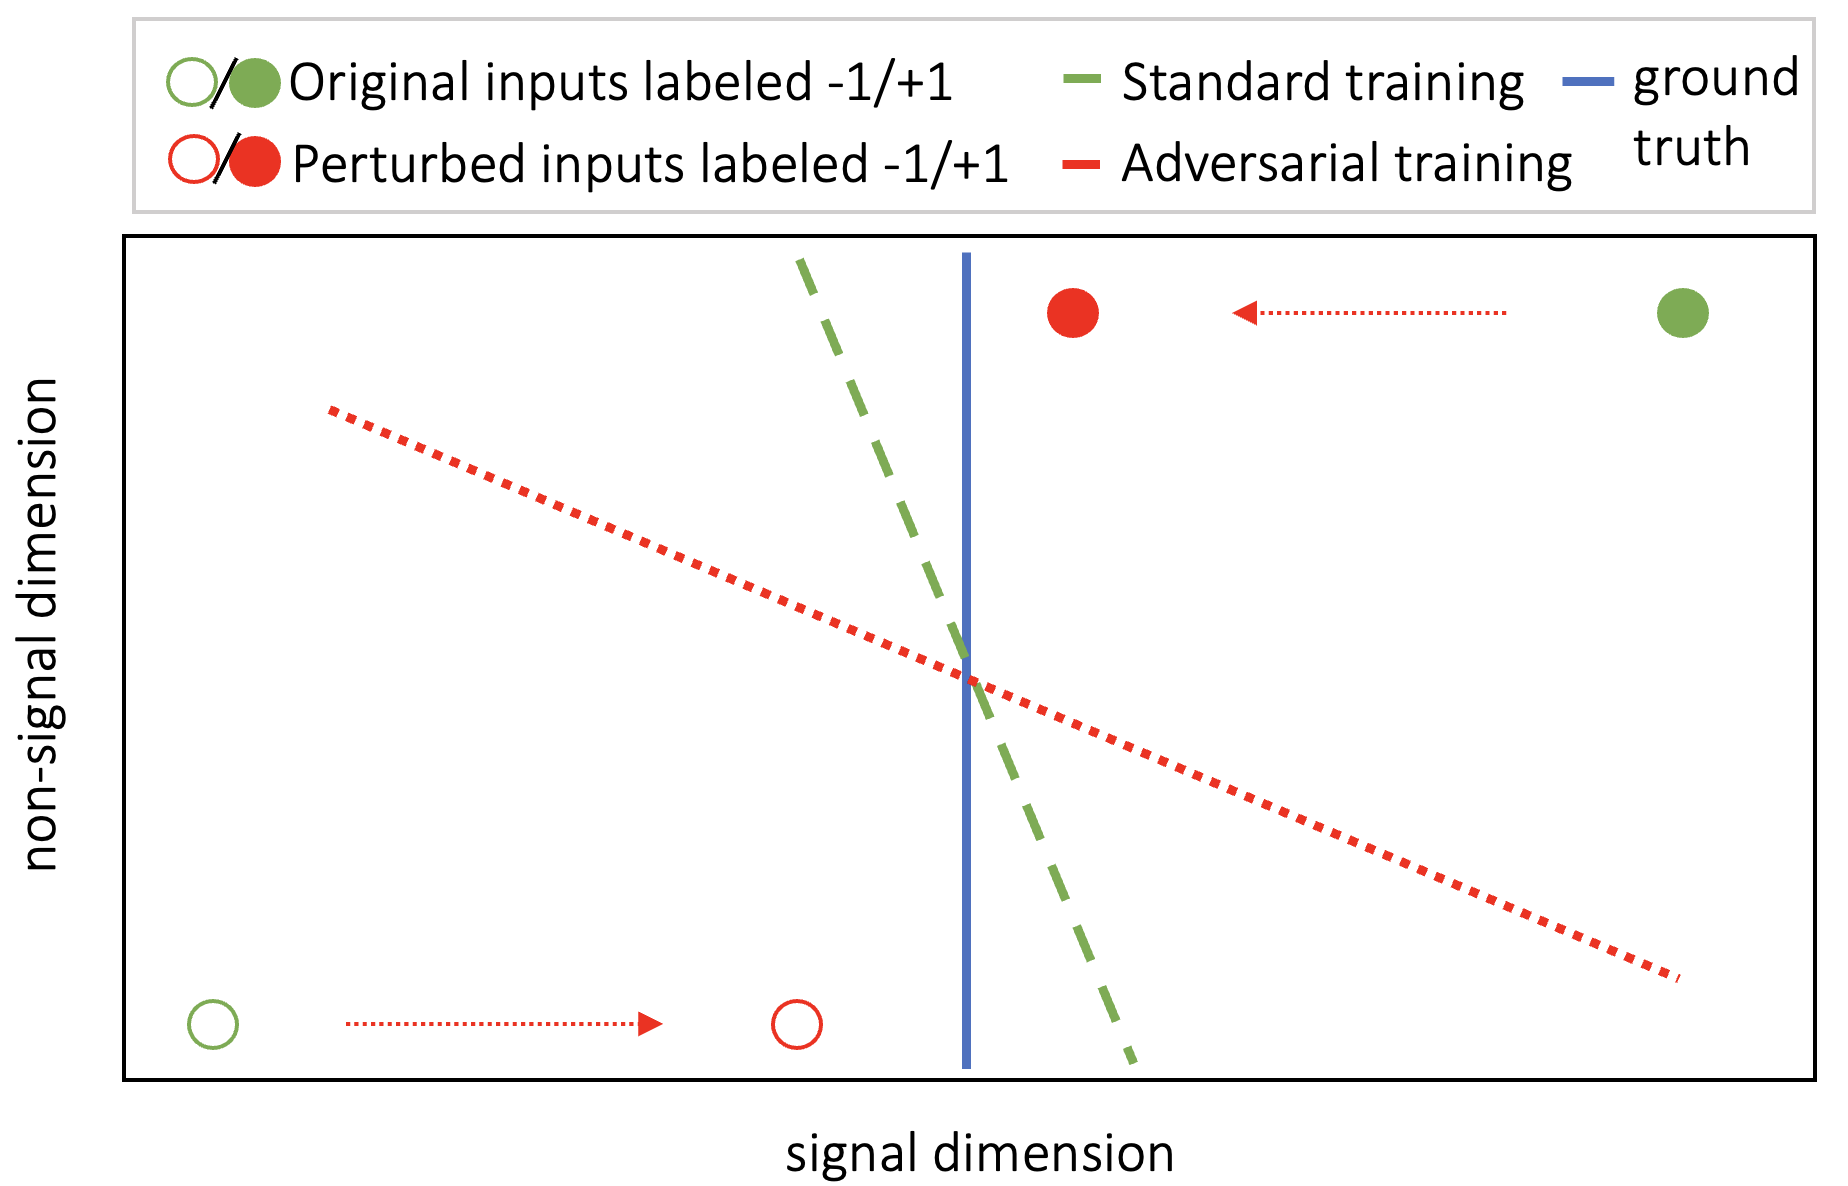
\includegraphics[width=0.99\linewidth]{plotsAistats/linear_intuition.png}
  %% \caption{ 2D illustration providing intuition for the linear example: Training on signal-attacking adversarial examples (red) effectively correspond to fiting the original datapoints (green) after shifted them closer to the decision boundary. The robust max-$\ell_2$-margin (red dotted) is heavily tilted if the points are far apart in the non-signal dimension, while the standard max-$\ell_2$-margin solution (green dashed) is much closer to the ground truth (blue solid).}

%%\label{fig:2D_dataset_intuition}
%%\end{figure}

The proof can be found in Appendix~\ref{sec:app_theorylinear} and
primarily relies on high-dimensional probability. Note that the
theorem holds for any $0\leq \epstest <\frac{\sigsep}{2}$ and hence
also directly applies to the standard error by setting $\epstest =
0$. In Figure~\ref{fig:main_theorem}, we empirically confirm the statements of Theorem \ref{thm:linlinf} by performing multiple experiments on synthetic datasets as described in Subsection \ref{logreg_linear_model} with different choices of $d/n$ and $\epstrain$. 
In the first statement, we prove that for small
sample-size ($n<d-1$) noiseless data,
%for small sample size settings $n<d-1$, 
%adversarial training hurts robust accuracy in the small sample regime
%for \emph{noiseless data}.
 %\fy{what we really prove is that lower and upper bound increase and expectation does, but} 
almost surely, the robust error increases monotonically with
adversarial training budget $\epstrain >0$. %with $\epstrain >0$ for noiseless data.
%% The same
%% holds almost surely for the high probability upper and lower bounds of
%% the robust error.
%% %% , adversarial
%% training with increasing $\epstrain$ monotonically increases.
%% This trend holds in expectation and for the
%% high probability upper and lower bounds.
%Experiments show that the trend holds with high probability
%within individual runs as well.
In Figure~\ref{fig:main_lower_bound_eps}, we plot the robust error gap between standard and adversarial logistic regression in function of the adversarial training budget $\epstrain$ for $5$ runs. 
%of $5$  independent experiments
%with datasets of size $n=50$ drawn according to the distribution $\prob_{\sigsep}$ with $\dims=1000,\sigma=1, \sigsep = 12$.
%% for
%% $\epstest>0$ and $\epstest=0$ (standard error) \fy{i still think
%%   standard accuracy is not important unless in the context of tradeoff
%%   we don't even mention it here} experimentally for $12$ independent
%% datasets of size $n=50$ drawn \fy{according to setting ref} with
%% $d=1000,\sigma=1$.
%that the trend holds with high probability within individual runs as well.

The second statement establishes a simplified lower bound on the
robust error increase for adversarial training (for a fixed
$\epstrain = \epstest$)  compared to standard training.
%We confirm this fact experimentally i
In Figures~\ref{fig:main_lower_bound_eps}  and \ref{fig:main_numobs_bound}, we show how the lower bound closely
predicts the robust error gap in our synthetic experiments.
%emphasize that this aligns with observations in real-world experiments \fy{ref to figures}. \fy{without the rest term I guess}
%% Note that as $\epstrain > \epscutoff$, the lower bound still monotically increases with $R(\epstrain,\epscutoff, \randvarphi) = \int_{\sigsep/2 -\epstrain}^{\sigsep/2 - \epscutoff} \frac{1}{\sqrt{2\pi} \randvarphi} \E^{-\frac{x^2}{\randvarphi^2}}$ \fy{but with a term that isn't clean and hence left out}.
Furthermore, by the dependence of $\varphimin$ on the overparameterization ratio $d/n$, the lower bound on the robust error gap is amplified for large $d/n$.
Indeed, Figure~\ref{fig:main_numobs_bound} shows how the error gap increases with $d/n$
both theoretically and experimentally. However, when $d/n$ increases above a certain threshold, the gap decreases again, as standard training fails to learn the signal and yields a high error (see Figure~\ref{fig:main_numobs}).
%% Furthermore, note that the assumption of linear separability in the $d-1$ last arguments shows how the phenomenon is intrinsically high-dimensional - as the sample size increases beyond $d-1$, the probability of linear separability drastically decreases and the detrimental effect of adversarial training fades.

%% shows the dependence of the drop
%% with respect to the sample size. In particular, it predicts that this
%% phenomenon is particularly severe in the high-dimensional, small
%% sample size regime when the ratio $\frac{d}{n}$ is large.

%% In
%% particular, $\varphimax, \varphimin$ arise from high probability
%% bounds on the largest eigenvalues of the empirical covariance matrix
%% and increase with $\frac{d}{n}$, thereby amplifying the robust error
%% increase with $\epstrain$. \fy{perhaps long}
%wherefore the increase of robust error with $\epstrain$ is amplified.



%% \fy{this thing is out of place: The tightness of the
%% bounds improves with increasing ratio $\frac{d}{n}$. }
%% the
%% experimental results indeed match the trends of our theoretical lower
%% and upper bound in Theorem~\ref{thm:linlinf}.

%\fy{kinda confused - for the expectation statement you can
 % compute it rigorously - i thought here you want to show
%  that each individual run (setting) also shows this trend - i.e.
%show 5 runs individually? } we can indeed do this!

%%   More precisely, as plotted in
%% Figure~\ref{fig:main_theorem}, increasing the perturbation set size
%% $\epstrain$ in the robust loss~\ref{eq:emploss} from standard training
%% ($\epstrain =0$) to $\epstest$ and beyond, the $\epstest$-robust
%% accuracy decreases monotonically. In particular, even when the
%% perturbations are consistent and the data is noiseless, adversarial
%% training with increasing $\epstrain$ monotonically decreases robust
%% generalization in our setting.


%\fy{for this I wonder if we should have average $\gamma$ as well}. No need I think
%% In particular, note that, for a fixed
%% large enough $\sigsep$, the decrease of robust accuracy with
%% $\epstrain$ is more severe for large $\maxmargin, \minmargin$
%% (i.e. small sample sizes $\numsamp$) by definition of the cumulative
%% distribution function.


%% our result
%% simultaneously extends the robustness and standard accuracy trade-off
%% result for linear regression \cite{raghunathan20} to linear
%% classification and uncovers an even more surprising phenomenon: that
%% adversarial training until convergence may in fact hurt robust
%% accuracy.

\begin{figure*}[!t]
\centering
\begin{subfigure}[b]{0.32\textwidth}
  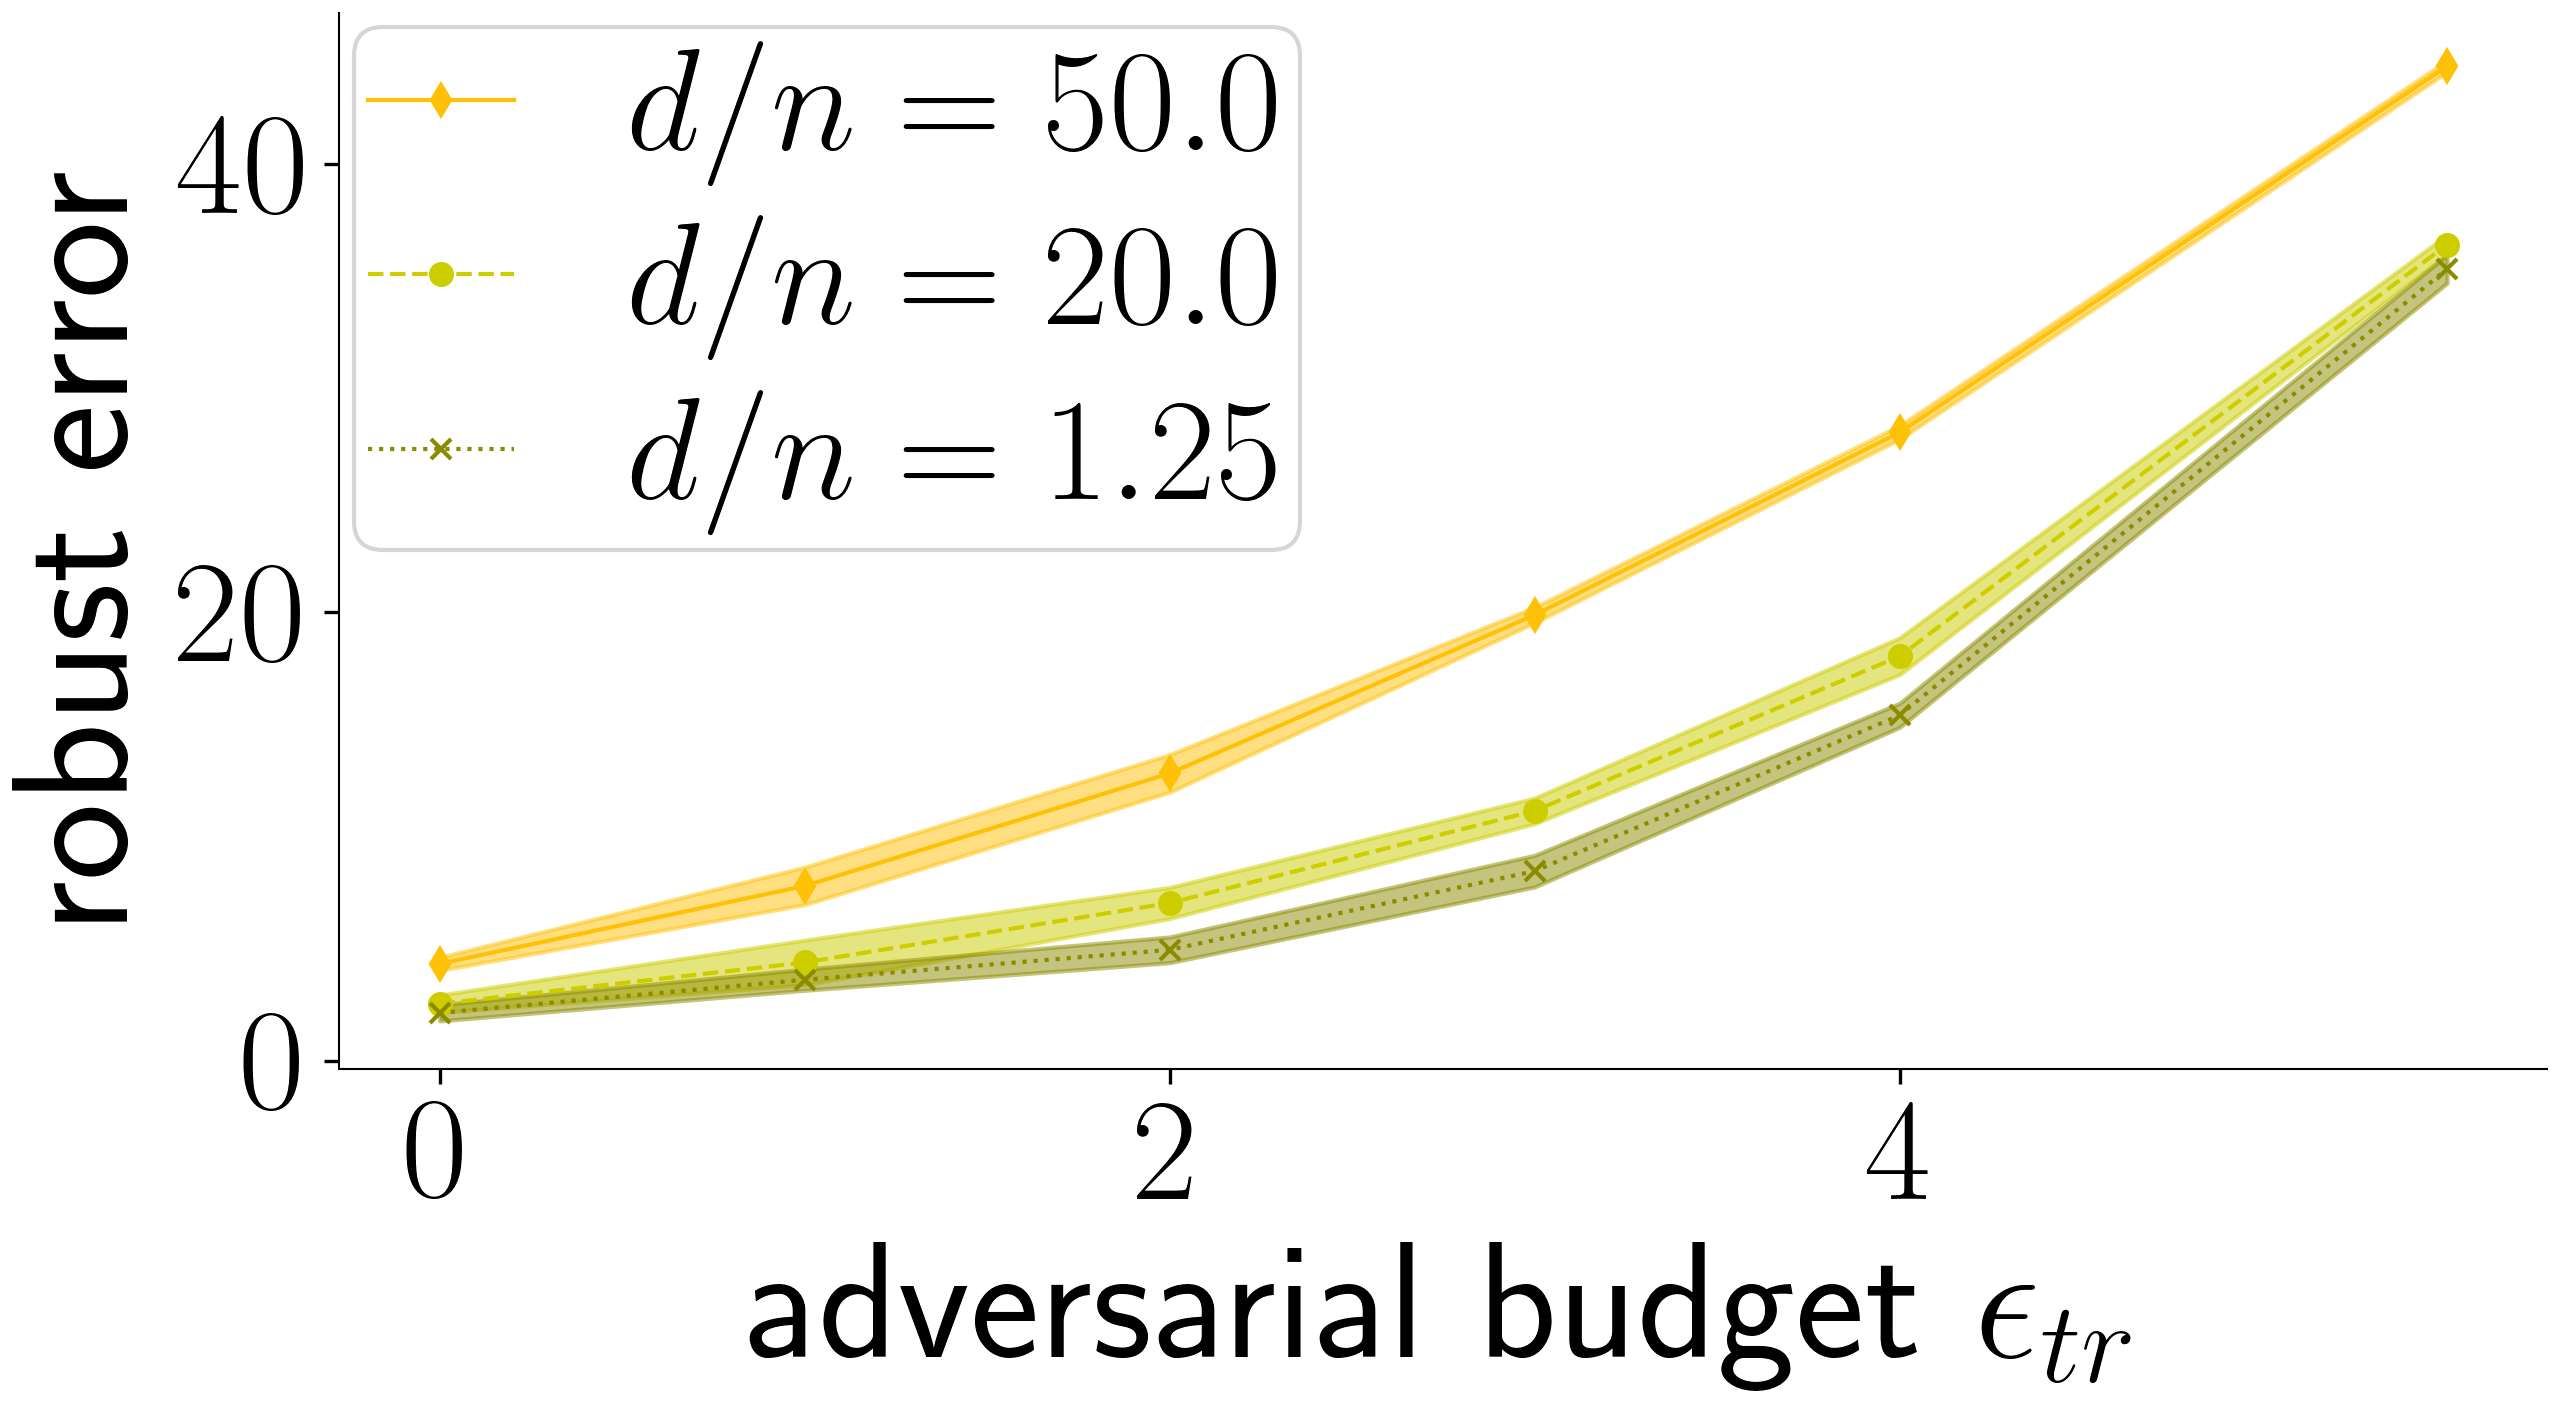
\includegraphics[width=0.99\linewidth]{plotsAistats/d_n_logreg.png}
  \caption{Robust error vs $\epstrain$}
  \label{fig:eps_logreg}
\end{subfigure}
\begin{subfigure}[b]{0.32\textwidth}
  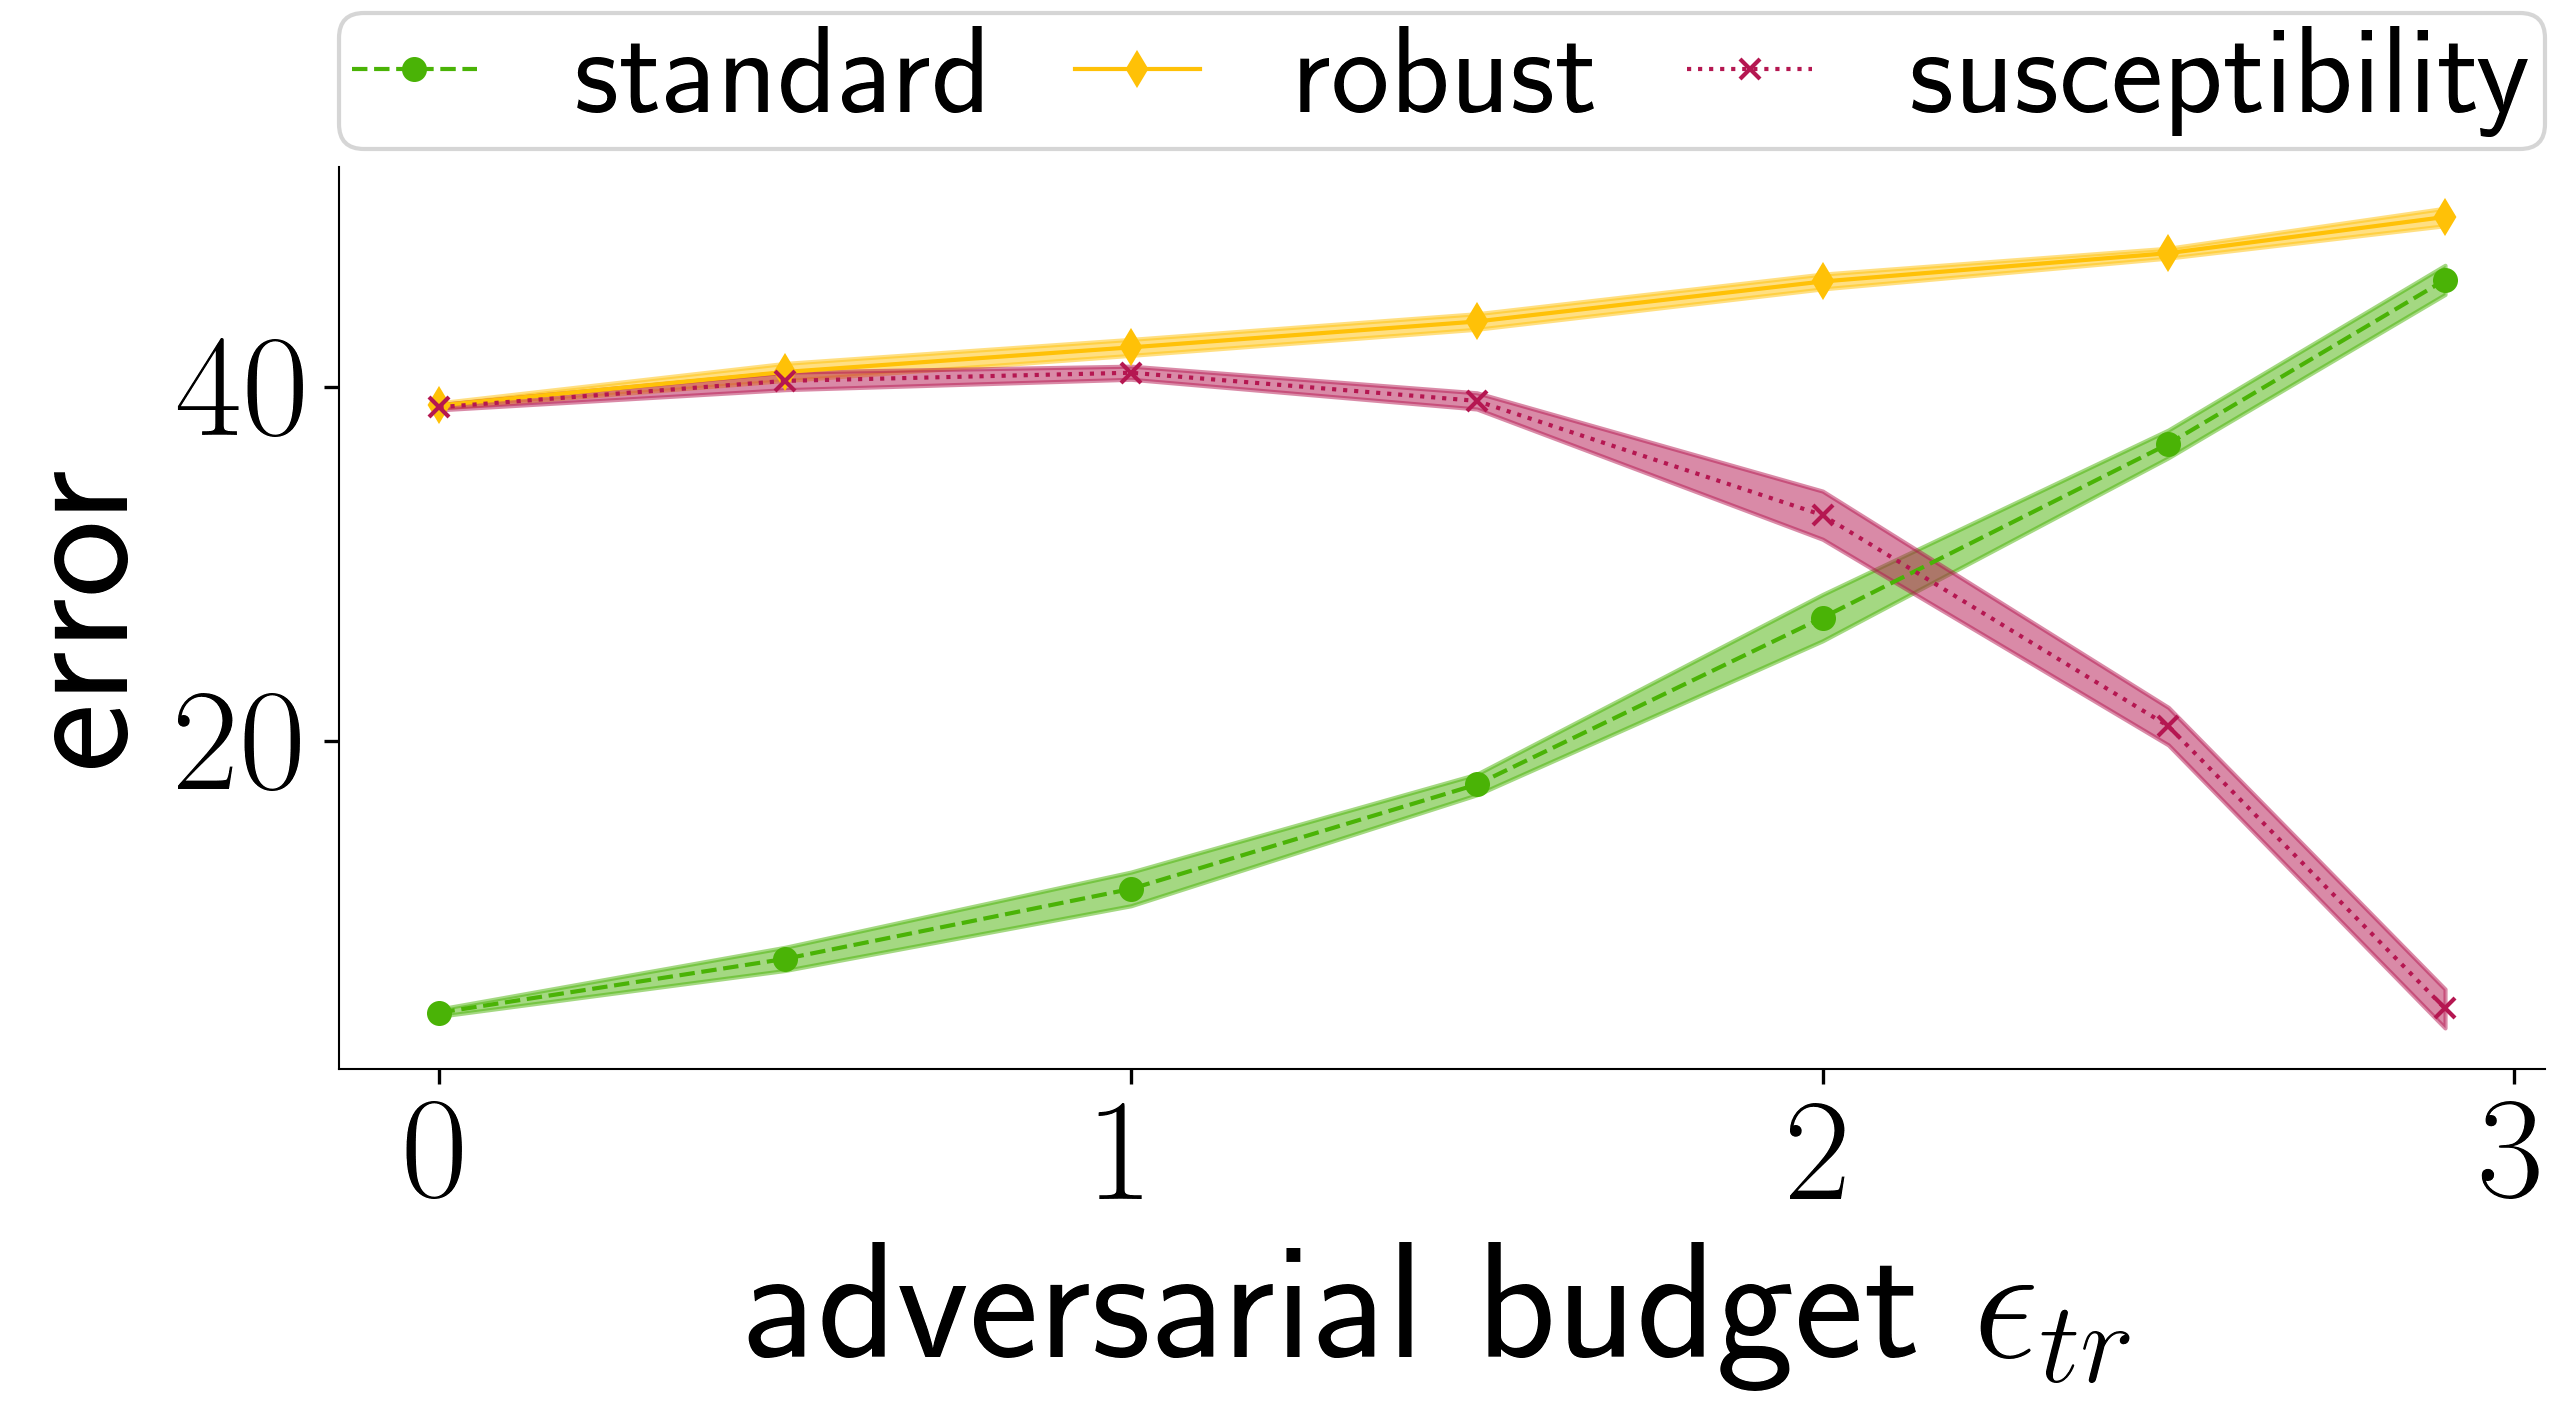
\includegraphics[width=0.99\linewidth]{plotsAistats/logreg_trade_off_plot.png}
  \caption{Robust error decomposition}
  \label{fig:main_robust}
\end{subfigure}
\begin{subfigure}[b]{0.32\textwidth}
  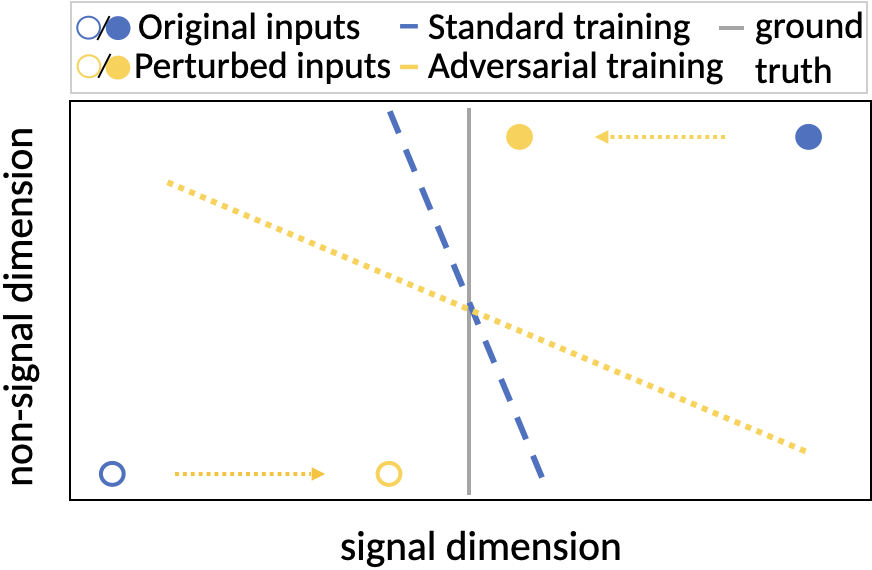
\includegraphics[width=0.99\linewidth]{plotsAistats/linear_intuition_try.png}
  \caption{Intuition in 2D}
  \label{fig:2D_dataset_intuition}
\end{subfigure}
\caption{(a) We set $\dims=1000$ and $\sigsep = 12$ and plot the robust error with increasing adversarial training budget ($\epstrain$) and with increasing $\dims/\numsamp$.  (b) We plot the robust error decomposition in susceptibility and standard error for increasing adversarial budget $\epstrain$. 
  %The increase in standard error dominates the drop in susceptibility leading to an increase in robust error.  
  Full experimental details can be found in Section~\ref{sec:logregapp}. (c) 2D illustration providing intuition for the linear setting: Training on \nameofattacks (yellow) effectively corresponds to fiting the original datapoints (blue) after shifting them closer to the decision boundary. The robust max-$\ell_2$-margin (yellow dotted) is heavily tilted if the points are far apart in the non-signal dimension, while the standard max-$\ell_2$-margin solution (blue dashed) is much closer to the ground truth (gray solid). }
\label{fig:lineartradeoff}
\end{figure*}

\subsection{Proof idea: intuition and surprises}
\label{logreg_proof_sketch}

The reason that adversarial training hurts
robust generalization is based on an extreme robust vs. standard
error tradeoff. We provide intuition for the effect of
\nameofattacks and the small sample regime
on the solution of adversarial training by decomposing the
robust error $\roberr{\theta}$.
Notice that $\epstest$-robust error $\roberr{\theta}$ 
can be written as the probability of the union of two events: the
event that the classifier based on $\theta$ is wrong and the event
that the classifier is susceptible to attacks:
\begin{equation}
 \label{eq:decomposition}
\begin{aligned}
     \roberr{\theta} &=  \EE_{x, y\sim \prob}  \left[\Indi{y f_\theta (x) <0} \vee \max_{x' \in \pertset{x}{\epstest}} \Indi{f_\theta(x) f_\theta(x')<0} \right] \\
  &\leq \stderr{\theta} + \suscept{\theta}
\end{aligned}
\end{equation}
where $\suscept{\theta}$ is the expectation of the maximization term in Equation \eqref{eq:decomposition}.
%% \begin{equation}
%%   \label{eq:robustness}
%% \suscept{\theta} : = \EE_{x\sim \prob} \max_{x'\in\pertset{x}{\epstest}} \Indi{f_\theta(x) f_\theta(x') <0}
%% \end{equation}
$\suscept{\theta}$ represents the $\epstrain$-\emph{attack-susceptibility} of a classifier
induced by $\theta$ and $\stderr{\theta}$ its standard error.
%with respect to an attack-model over the data distribution $\prob$.
Equation~\eqref{eq:decomposition} suggests that
the robust error can only be small if both the standard error and
susceptibility are small. In Figure~\ref{fig:main_robust}, we
plot the decomposition of the robust error in standard error and susceptibility for adversarial logistic regression with increasing $\epstrain$. We observe that increasing $\epstrain$
increases the standard error too drastically compared to the decrease
in susceptibility, leading to an effective drop in robust accuracy. For completeness, in Appendix \ref{app:susc}, we provide upper and lower bounds for the susceptibility score.  We
now explain why, in the small-sample size regime, adversarial training
with \nameofattacks ~\eqref{eq:linfmaxpert} may increase standard
error to the extent that it dominates the decrease in susceptibility.
%even though robustness increases with $\epstrain$,
% dominates the increase in robustness thereby 


%% robust accuracy $\robacc{\theta} = 1- \roberr{\theta}$.
%% %% In what follows we focus on accuracy, that is for a
%% %% linear classifier induced by $\theta$, we define the accuracy as $
%% %% \robacc{\theta} = 1- \roberr{\theta}$.
%% In particular, notice that $\epstest$-robust accuracy $\robacc{\theta}$ 
%% can be written as the probability of the intersection of two events: the
%% event that the classifier based on $\theta$ is correct and the event
%% that the classifier is robust
%% \begin{equation}
%% \begin{aligned}
%%   \label{eq:decomposition}
%%      &\robacc{\theta}= \\
%%     &\EE_{x, y\sim \prob}  \Indi{y f_\theta (x) >0} \min_{x' \in \pertset{x}{\epstest}} \Indi{f_\theta(x) f_\theta(x')>0}. \nonumber
%% \end{aligned}
%% \end{equation}
%% We refer to the expectation of the inner minimization term

%% \begin{equation}
%%   \label{eq:robustness}
%% \robness{\theta} : = \EE_{x\sim \prob} \min_{x'\in\pertset{x}{\epstest}} \Indi{f_\theta(x) f_\theta(x') >0}
%% \end{equation}
%% as the \emph{robustness} of a classifier induced by $\theta$ with
%% respect to an attack-model over the data distribution $\prob$.

%On the other hand, the expectation of the first factor $\EE_{x, y\sim \prob}
%\Indi{y f_\theta (x) >0}$ corresponds to the standard err $\stderr{\theta}$.
%% The accuracy can only be large if both standard accuracy and
%% robustness are large. In Figure~\ref{fig:lineartradeoff} a), we plot
%% the decomposition and observe that even though robustness increases
%% with $\epstrain$, the decrease in standard accuracy dominates the
%% increase in robustness thereby leading to an effective drop in robust
%% accuracy.


%and robust accuracy despite increasing robustness in the high-dimensional regime.

%% \fy{which?} happen with the signal-directed perturbation
%% set~\eqref{eq:linfmaxpert} first using an illustration and then using
%% intermediate results used in the proof.
%% We provide some intuition behind the main steps in the proof of
%% Theorem~\ref{thm:linlinf} for 
%The full proof can be found in Section~\ref{sec:app_theorylinear}.

A key observation is that the robust max-$\ell_2$-margin solution of a
dataset $\data= \{(x_i, y_i)\}_{i=1}^n$ 
%defined in~\eqref{eq:maxmargin} 
maximizes the minimum margin that reads ${\min_{i\in [n]}
  y_i \theta^\top (x_i - y_i \epstrain |\thetaind{1}| e_1)}$, where
$\indof{\theta}{i}$ refers to the $i$-th entry of vector $\theta$. Therefore, it
simply corresponds to the max $\ell_2$-margin solution of the dataset
shifted towards the decision boundary ${\Dshift = \{(x_i - y_i \epstrain
  |\indof{\thetahat{\epstrain}}{1}| e_1, y_i)\}_{i=1}^n}$.
%that is the original training set $\data$ shifted by $\epstrain$ in
%the first dimension.
Using this fact, we obtain 
a closed-form expression of the (normalized) max-margin solution~\eqref{eq:maxmargin} as a function of
$\epstrain$ that reads
\begin{equation}
  \label{eq:maxmarginmaintext}
\thetahat{\epstrain} = \frac{1}{(r-2\epstrain)^2 + 4 \marginnonsig^2}
\left[\sigsep - 2\epstrain, 2 \marginnonsig \thetatilde \right],
\end{equation} 
% normalized versions of $\left[\sigsep - \epstrain, 2 \marginnonsig \thetatilde \right]$,
where $\|\thetatilde\|_2 = 1$ and $\marginnonsig >0$ is a random quantity
associated with the max-$\ell_2$-margin solution of the
$\dims-1$ dimensional Gaussian inputs orthogonal
to the signal direction
(see Lemma~\ref{lem:maxmargin} in Section~\ref{sec:app_theorylinear}).

In high dimensions, with high probability any two
Gaussian random vectors are far apart -- in our
distributional setting, this corresponds to the vectors being far
apart in the non-signal directions. In
Figure~\ref{fig:2D_dataset_intuition}, we illustrate the phenomenon
using a simplified 2D cartoon, where the few samples
in the dataset are all far apart in the non-signal direction.
We see how shifting the dataset closer to the true decision boundary,
%% small sample sizes relative to the intrinsic
%% dimension, this intuition might fail: a training set closer to the
%% decision boundary results
may result in a max-margin solution (yellow) that aligns much worse
with the ground truth (gray), compared to the estimator learned from
the original points (blue). Even though the new (robust max-margin)
classifier (yellow) is less susceptible to directed attacks in the
signal dimension, it also uses the signal dimension less.
%, corresponding to a more tilted decision boundary.  
Mathematically, this is directly
reflected in the expression of the max-margin solution in
Equation~\eqref{eq:maxmarginmaintext}: Even without the definition of
$\marginnonsig, \thetatilde$, we can directly see that the first
(signal) dimension is used less as $\epstrain$ increases.
%; the
%classifier relies more on the non-signal dimensions to classify the training data.(tautorical)



%% the non-useful features dominate the learned classifier
%% and hence 
%% we are putting more weight on robust, but non-useful features.
%% This effect increases with the ratio $\frac{d}{n}$ via
%% the random quantity $\marginnonsig$ that is upper and lower bounded by
%% $\maxmargin, \minmargin$.


%% \fy{In particular, note that for directed attacks, this trade-off is unavoidable (in which sense) ... see proof? there's no way to change one independent from another - instead of this:}
%% In comparison to previous scenarios where the trade-off was studied, intuitively the drop in standard accuracy dominates the trade-off for \nameofattacks more severely, because they are more directly targeting the signal.

%% I.e. it uses the signal dimension less. The same mechanism, however, increases robustness to increase against attacks in said direction.
%\fy{hence intrinsically at odds}



%% Now note that in line with the definition of \nameofattacks, this
%% shifted dataset is closer to the decision boundary of the ground truth
%% $\thetatrue$. The usual intuition from low-dimensional problems
%% suggests that few samples close to the true decision boundary would
%% yield a better estimator compared to the same number of samples far
%% from the boundary.


%% For our data generating model in Section~\ref{sec:} we can show that 
%% that with probability
%% at least $\E^{-\tconst^2 (\dims-1)/2}$,
%% \begin{equation}
%%   \label{eq:gammasandwich}
%%   (1+\tconst)\sqrt{\frac{\dims-1}{\numsamp}} + 1 \leq \frac{\marginnonsig}{\mixvar} \leq (1-\tconst) \sqrt{\frac{\dims-1}{\numsamp}}-1.
%% \end{equation}
%% And hence, the larger $d/n$, the bigger the effect.

%\fy{this could be moved to appendix if little space}
%% This intuition can also be quantified mathematically using
%% intermediates results in the proof of our theorem.  First of all,
%% Lemma~\ref{lem:maxmargin} in Section~\ref{sec:app_theorylinear}
%% provides the closed-form expression of the max-margin classifier
%% $\thetahat{\epstrain} = \frac{1}{(r-2\epstrain)^2 + 4 \marginnonsig^2}
%% \left[\sigsep - 2\epstrain, 2 \marginnonsig \thetatilde \right]$, 
%%  normalized versions of $\left[\sigsep - \epstrain, 2 \marginnonsig \thetatilde \right]$,
%% where $\|\thetatilde\|_2 = 1$ and $\marginnonsig$ is a random quantity
%% depending on the last $\dims-1$ dimensions of the inputs.
%% Even without the definition of $\marginnonsig, \thetatilde$, we can
%% directly see from the expression how the first (signal) dimension is
%% less used as $\epstrain$ increases and the classifier relies on the
%% non-signal dimensions more heavily. In the words of \cite{ilyas19, springer21},
%% we are putting more weight on robust, but non-useful features.

%% NOTE::: perhaps could still use a proof sketch thing in the appendix? or erase.
%% this occurs with
%% high probability if the data is in a high dimensional regime: standard
%% Gaussian vectors (that constitute the $d-1$ dimensions of our input
%% not being used by the ground truth) are close to being uniformly
%% distributed on a sphere of radius $\sqrt{d}$ (see
%% e.g.\cite{vershynin18}). Hence, in the $d-1$ non-signal dimensions of
%% an input in our dataset, any relatively small set of $\numsamp \ll
%% \dims$ points is comprised of vectors that are far apart.
%% \fy{somehow this sounds very particular to the gaussian distribution}


%% In order to make this intuition quantitive, in the proof we bound the random
%% quantities $\marginnonsig, \thetatilde$ in the closed-form solution of
%% the robust max-margin soution. Using matrix concentration results for
%% Gaussian matrices stated in Lemma~\ref{lemma_bounding_gamma} in
%% Section~\ref{sec:sandwichmarginproof}, we obtain that with probability
%% at least $\E^{-\tconst^2 (d-1)/2}$,
%% \begin{equation}
%%   \label{eq:gammasandwich}
%%   (1+\tconst)\sqrt{\frac{\dims-1}{\numsamp}} + 1 \leq \frac{\marginnonsig}{\mixvar} \leq (1-\tconst) \sqrt{\frac{\dims-1}{\numsamp}}-1.
%% \end{equation}
%% On the other hand, by definition of the test distribution
%% $\prob_\sigsep$, a small calculation yields that the $\epstest$-robust
%%   accuracy can be written as $\Phi\left(\frac{(\sigsep -
%%     2\epstrain)(\sigsep-2\epstest)}{4\mixvar \marginnonsig} \right)$ (as derived in Equation~\ref{eq:robacc_closed} in Section~\ref{sec:thmproof})
%%   and the Gaussian cumulative distribution function, it follows
%%   directly. The theorem statement then follows by combining 
%%   this expression with Equation~\ref{eq:gammasandwich}.



\subsection{Generality of the results}

In this section we discuss how the theorem might generalize to
other perturbation sets, models and training procedures.
\paragraph{Signal direction is known}
The type of additive perturbations used in Theorem~\ref{thm:linlinf},
defined in Equation~\eqref{eq:linfmaxpert}, is explicitly constrained
to the direction of the true signal. This choice is reminiscent of
corruptions where every possible perturbation in the set is directly
targeted at the object to be recognized, such as motion blur of moving
objects.  Such corruptions are also studied in the context of domain
generalization and adaptation \cite{Schneider20}.
%% The only search is within the severity of the perturbation
%% via $\epstest$.  For such perturbations, clearly, the biggest
%% perturbation should also be the worst - so effectively we might not
%% really need a search except for nonconvexity reasons \cite{yang19,
%%   engstrom19}. In the literature there are variants where one augments
%% with random augmentation \cite{hendrycks20} or with the most extreme
%% augmentation \cite{calian21}.

\nameofattackscapital in general, however, may also consist of
perturbation sets that are only strongly biased towards the true
signal direction, such as mask attacks.  They may find the true signal
direction only when the inner maximization is
exact. The following corollary extends Theorem~\ref{thm:linlinf} to
small $\ell_1$-perturbations
\begin{equation}
  \label{eq:l1maxpert}
  \pertset{x}{\eps} = \{x'=x+\delta \mid \|\delta\|_1 \leq \eps\},
\end{equation}
for $0<\eps<\frac{\sigsep}{2}$ that reflect such attacks. We state the corollary here and give the proof in Appendix \ref{sec:app_theorylinear}.
%The extension is summarized in the following corollary
%% In the following corollary
%% we show that our theorem also holds for ``real search'' perturbation
%% sets such as bounded $\ell_1$-balls
\begin{corollary}
\label{cor:l1extension}
  Theorem~\ref{thm:linlinf} also holds for ~\eqref{eq:maxmargin} with perturbation sets defined in \eqref{eq:l1maxpert}.
\end{corollary}
The proof uses the fact that the inner maximization
effectively results in a sparse perturbation equivalent to the attack
resulting from the perturbation set~\eqref{eq:linfmaxpert}. 

%\paragraph{Feature learning}
%Wen now argue that the intuition that in high-dimensions adversarial
%training puts more weight on learning robust features that are all
%non-useful for \nameofattacks , carries over to feature learning
%models.  First, we show how adversarial training indeed hurts robust
%generalization when we train a simple 2-layer neural network with
%quadratic activations to fit a high-dimensional concentric spheres
%dataset, where the signal feature is the norm only.
%We then demonstrate experimentally how adversarial training indeed leads to hyperboloid instead of ellipsoid decision boundaries -- that is, as $d>n$
%the adversarially trained classifier uses robust but non-useful features instead \fy{this seems to me only meaningful if it gets more severe with d/n else its ilyas, maybe have d/n <1 as well to show it doesn't happen there}.
%\fy{can we see why hyperboloid bla is more likely if $d/n$ large? else the ``intuition'' is not new (follows directly from ilyas) plus disscimilarity score plot isn't really showing a very clear trend for large epstrain, pick what you plot}

%% In order to argue that the intuition gained by the linearmodel \fy{which? that you learn robust non-useful features more? but that highlevel can already be deduced by ilyas} in
%% this section may also at least partially explain the real-world
%% experiments with neural networks, in Appendix~\ref{sec:app_theorycs}
%% we also train a simple 2-layer neural network with quadratic
%% activations to fit a high-dimensional concentric spheres dataset.
%% We first show that the  also happens
%% when the neural network is trained to fit concentric spheres
%% where the signal feature is the norm only.
%% We formalize how adversarial
%% training in the low sample regime causes the neural networks to use
%% robust but non-useful features to classify the training points by
%% analysing \fy{what does analyze mean} the decision boundaries of the networks. We
%% plot in Figure \ref{fig:eps_cs} the result of different runs on the
%% synthetic dataset and recognize that especially in the low sample size
%% regime, adversarial training hurts robust generalization.

%% We would like to note that we can verify a similar statement and its
%% intuition for feature learning such as with neural networks by
%% analysing the decision boundary and robust accuracy of the converged
%% models. In Appendix \ref{sec:app_theorycs} we discuss a case with a
%% 2-layer neural network with quadratic activations.
%% In Figure
%% \ref{fig:eps_cs}, we plot the robust accuracy with increasing
%% $\epstrain$ and notice the similarity with the linear case, plotted in
%% Figure \ref{fig:eps_logreg}.

\paragraph{Other models}
Motivated by the implicit bias results of (stochastic)
gradient descent on the logistic loss, Theorem~\ref{thm:linlinf} is proven for the max-$\ell_2$-margin
solution. We would like to conjecture
that for the data distribution in Section \ref{sec:theoryresults},
adversarial training can hurt robust generalization also for other models with zero
training error (\emph{interpolators} in short).

%% minimizes
%% the training objective \fy{interpolates the data - maybe a bit strong, just l1 for now?}.
For example, Adaboost is a widely used algorithm that converges to the max-$\ell_1$-margin classifier \cite{telgarsky13}. One might argue that for a sparse ground truth, the max-$\ell_1$-margin classifier should (at least in the noiseless case) have the right inductive bias to alleviate large bias in high dimensions. Hence, in many cases the (sparse) max-$\ell_1$-margin solution might align with the ground
truth for a given dataset. However, we conjecture that even in this
case, the \emph{robust} max-$\ell_1$-margin solution (of the dataset
shifted towards the decision boundary) would be misled to choose a
wrong sparse solution. This can be seen with the help of the cartoon
illustration in Figure \ref{fig:2D_dataset_intuition}.

%% using the cartoon illustration, one can easily see how \nameofattacks could bias the classifier towards a wrong (albeit sparse) solution.

%% a similar result can be proven for the max-$\ell_1$-margin
%% solution that results from training with AdaBoost.
%% Clearly, even though the max-$\ell_1$-margin solution usually outperforms the max-$\ell_2$-margin solution, using the cartoon illustration, one can easily see how \nameofattacks could bias the classifier towards a wrong (albeit sparse) solution.
%% The general intuition can be understood using the taxonomy of \cite{ilyas19}: all useful features, which have a non-zero correlation with the true labels, whether robust or not, are reduced in strength by \nameofattacks :the correlation strength reduces. On the other hand, all non-useful features remain untouched. Hence, the classifier relies more on non-useful features to classify the training dataset.

%%The general intuition can be stated using the taxonomy
%%introduced by \cite{ilyas19}: 
%%by definition none of the useful features but non-robust features can be robust with %%%respect to \nameofattacks. However, \nameofattacks also decreases the strength of %%the robust but useful features. 
%%However, \nameofattacks biases the classifier
%%towards using robust and hence non-useful features \emph{independent} of the 
%%original bias. Hence, requiring robustness against \nameofattacks during training can %%only bias the solution away from the structure of the ground truth, which is 
%%particularly hurtful in the low sample regime.


%% However, even with an max $\ell_1$-margin bias, the phenomenon of adversarial training hurting robust generalization persists. It does not matter with which interpolator you start with as signal-attacking perturbations bias any interpolator away from the ground truth, which hurts robust generalization.

